\chapter{増幅器の効果}
減衰通信路に増幅器を設置する効果について評価を行う。
増幅器の設置位置としては減衰通信路のちょうど真ん中に設置する場合と、受信器の直前に設置する場合について考える。
以下は増幅器を減衰通信路のちょうど真ん中に設置する場合の減衰+増幅+減衰のプログラムである。
\begin{lstlisting}[caption=減衰+増幅+減衰のプログラム,label=program6]

att_rate_total=0.9
att_rate=np.sqrt(att_rate_total)
gain=1/att_rate
for j in range(M):
  output_qstates[j].attenuate(att_rate)
  output_qstates[j].amplificate(gain)
  output_qstates[j].attenuate(att_rate)

\end{lstlisting}

また、以下は更に前置増幅器も設置する場合の、減衰+増幅+減衰+
前置増幅のプログラムである。

\begin{lstlisting}[caption=減衰+増幅+減衰+前置増幅のプログラム,label=program7]

att_rate_total=0.9
att_rate=np.sqrt(att_rate_total)
gain=1/att_rate
for j in range(M):
  output_qstates[j].attenuate(att_rate)
  output_qstates[j].amplificate(gain)
  output_qstates[j].attenuate(att_rate)
  output_qstates[j].amplificate(gain)

\end{lstlisting}


次に、増幅器を減衰通信路の中間位置においた場合の評価を行う。また、前置増幅を行った場合と前置増幅を行わず強度調整を行った場合の比較も合わせて行うことにする。\figref{Fig:5_5}は信号の最大強度が5、基底数が256、送信データ数が1000個の場合に透過率と正規受信者の誤り率の関係を表したものである。

本実験では、信号が受信される直前に増幅をさせる(前置増幅)。増幅のみを行った場合に比べると誤り率は低く見られたが増幅と信号強度の調整を行った場合に比べると誤り率は少し高くなっている。

\begin{figure}[htbp]
        \centering   
        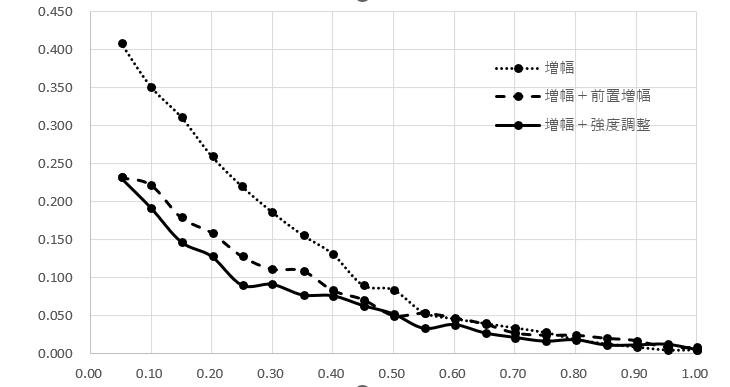
\includegraphics[width=1\textwidth]{img/zemi1-2.png}
        \caption[sample image (png)]{前置増幅と誤り率の関係.}
        \label{Fig:5_5}
    \end{figure}